\section{Колебания и дифференциальные уравнения}
\epigraph{\textsf{May the force be with you.}}{\texttt{Everybody from SW.}}
Перейдем к кульминации всего курса - составлению дифференциальных уравнений (уравнения на функцию, где фигурирует ее производная), которые являются неотъемлемой частью познания физических законов. Не будем перегонять из пустого в порожнее!
\subsection{Формула Циолковского}
\begin{figure}[h!]
    \centering{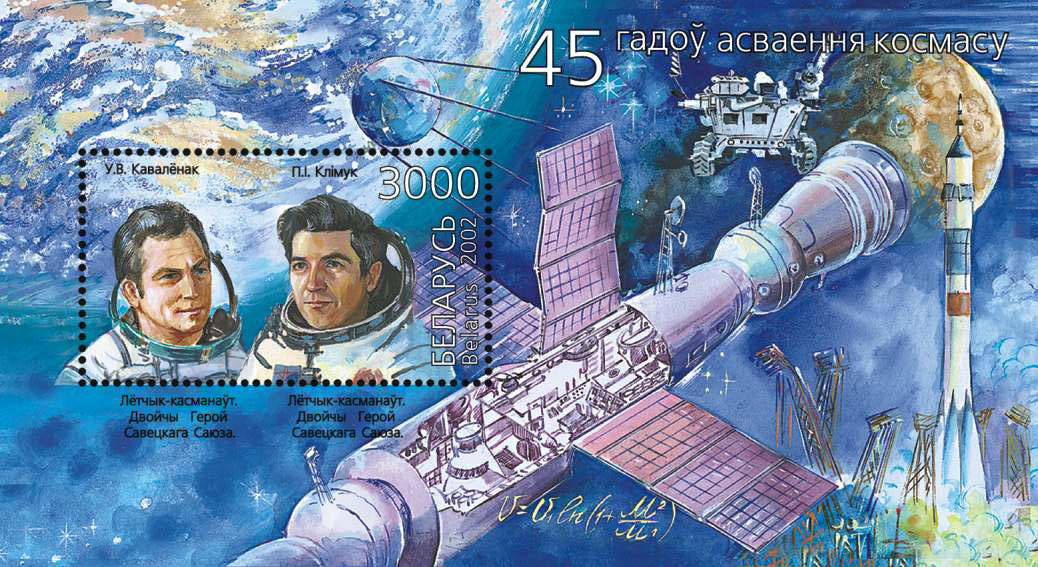
\includegraphics[scale=0.2]{pics/rocket.jpg}}
    \caption{Уравнение Циолковского на марке}
\end{figure}

Рассмотрим движение ракеты в космосе.
Сначала пренебрежём всеми внешними силами, действующими на ракету. Основными параметрами, характеризующими ракету и её двигатель, являются: $\boldsymbol{u}_0$ — скорость истечения газов из сопла ракеты относительно корпуса ракеты, для простоты считаем её постоянной, $M_0$ — исходная масса ракеты с горючим, $M_{\text{к}}$ — конечная масса ракеты после выгорания всего горючего.

Ракета имеет скорость $v$, массу $M$ в момент времени $t$. Выбрасывается топливо массы $\Delta M$ со скоростью $u_0$. Импульс сохраняется, тогда 
\begin{equation*}
    Mv = (M - \Delta M)(v + \Delta v) + \Delta M (v + u_0)
\end{equation*}

Тогда получим дифференциального уравнение 1-го порядка (фигурирует производная 1-ой степени)
\begin{equation*}
    M\Delta v =  - \Delta M u_0 \Rightarrow v(t) = - u_0 \int_{M_0}^{M_\text{к}} \frac{dM}{M}
\end{equation*}
Этот сделан предварительно перейдя к дифференциалам. Итого
\begin{equation*}
    v = u_0 \ln \Bigl(\frac{M_0}{M_{\text{к}}} \Bigr)
\end{equation*}
Таким образом, скорость ракеты увеличивается с уменьшением массы ракеты!!! Именно поэтому мы грузим топливо в ракеты, а не просто запускаем их из, например, рогатки.
\subsection{Почему Коши оказался в диффурах?}
Теперь зададимся вопросом - почему дифференциальные уравнения (вообще любые) имеют решения при должном числе условий, наложенных на функцию? Оказывается, что ответ на этот вопрос был дан довольно-таки давно. Задачи, где дано дифференциальное уравнение и условие на функцию, называют \textit{задачами Коши}. Например, уравнение Циолковского
\begin{equation*}
    \begin{cases}
        \frac{dv}{dM}= - \frac{u_0}{M}\\
        v(M = M_0) = 0
    \end{cases}
\end{equation*}

Так оказывается, что такие задачи \textbf{всегда} имеют решение!
\begin{theorem}(Теорема о разрешимости задачи Коши)
    Пусть есть поставленная задача Коши на отрезке
    \begin{equation*}
        \begin{cases}
            y^{'} = f(x,y),\ x \in (x_0, a]\\
            y^{'}(x_0) = y^{0}
        \end{cases}
    \end{equation*}
    Тогда, если функция $f(x,y)$ удовлетворяет (\dots \textbf{куча условий} \dots), то решение \textbf{существует} и \textbf{единственно}.
\end{theorem}
Подробнее об этом вам расскажут в университете, поэтому на этом мы внимание заострять не будем. Зато теперь мы решаем дифференциальные уравнения законно!
\subsection{Математический маятник: чем больше тел, тем сложнее путь}
Теперь попробуем решить задачу для колебания математического маятника.
\begin{figure}[h!]
    \centering{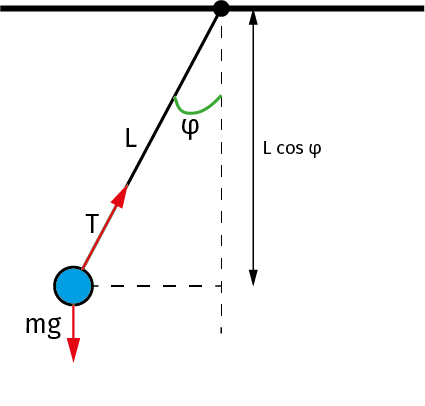
\includegraphics[scale = 1]{pics/mat_mayatnik.png}}
    \caption{Математический маятник.}
\end{figure}

Поступим следующим образом: запишем полную энергию системы а потом уже найдем силу, действующую на груз. Сначала перейдем к углу отклоения $\phi$ и выразим все через него. Таким образом
\begin{equation*}
    y = -L\cos \phi,\ x = L \sin \phi
\end{equation*} 

Полная энергия системы равна
\begin{equation*}
    W = \frac{m L^2 \dot{\phi}^2}{2} - mgL \cos \phi
\end{equation*}
Теперь запишем теорему, которая нам пригодится
\begin{theorem}(Связь силы и поля)
    Равнодействуйющая всех сил, действующих на систему, связаны с потенциальной энергией $U$ следующим соотношением
    \begin{equation*}
        F_x = -\frac{\partial U}{\partial x},\ F_y = -\frac{\partial U}{\partial y},\ F_z = -\frac{\partial U}{\partial z} \Rightarrow \vec{F} = - \nabla U
    \end{equation*}
    где значок $\nabla$ - называется \textbf{наблой}, и под собой подразумевает $\nabla = \{\frac{\partial}{\partial x},\frac{\partial}{\partial y}, \frac{\partial}{\partial z} \}$
\end{theorem}
\begin{proof}
    Так как $dA = (\vec{F}, d \vec{r})$, а $dA = - dU$, то 
    \begin{equation*}
        dU = -(\vec{F}, d \vec{r}) = - F_x dx - F_y dy - F_z dz \Rightarrow F_{\alpha_i} = - \frac{\partial U}{\partial \alpha_i},\ \alpha_i = {x, y, z}
    \end{equation*}
    И тогда $\vec{F} = - \nabla U$
\end{proof}
Так как мы "сидим"\ в угловых координатах, то изменение положения маятника будет происходить по дуге. Тогда
\begin{equation*}
    m a_{\text{ц.с.}} = m l \ddot{\phi} = - \frac{\partial U}{L \partial \phi} = mg \frac{\partial \cos \phi}{\partial \phi } = - mg \sin \phi
\end{equation*}

Таким образом
\begin{equation*}
    \ddot{\phi} = - \frac{g}{L} \sin \phi
\end{equation*}
Если воспользоваться допущением, что угол отклонения $\phi$ мал, то мы получим
\begin{equation*}
    \ddot{\phi} = - \frac{g}{L} \phi \Rightarrow \ddot{\phi} + \omega^2 \phi = 0,\ \omega = \sqrt{\frac{g}{L}}
\end{equation*}
Решением такого дифференциального уравнения являются гармонические функции
\begin{equation*}
    \phi(t) = A \cos (\omega t) + B \sin (\omega t)
\end{equation*}
где $A$ и $B$ можно найти из начальных условий. 

Данную задачу можно было решить по другому, если бы мы спроецировали силу тяжести на ось, перпендикулярную нити
\begin{equation*}
    m a_{\tau} = m l \ddot{\phi}  = - mg\sin \phi
\end{equation*}

\subsection{Гармонический осциллятор}
Рассмотрим еще один известнейший маятник - пружинный. 

\begin{figure}[h!]
    \centering{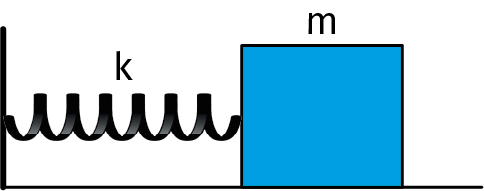
\includegraphics[scale=0.7]{pics/pruz_mayatnik.png}}
    \caption{Пружинный маятник.}
\end{figure}

Запишем второй закон Ньютона при отклонении на малую величину $x$
\begin{equation*}
    m\ddot{x} = \Bigl(kx_0 - k(x + x_0) \Bigr) = - kx \Rightarrow \ddot{x} + \omega^2 x = 0,\ \omega = \sqrt{\frac{k}{m}}
\end{equation*}

Давайте запишем полную энергию маятника
\begin{equation*}
    W = \frac{m \dot{x}^2}{2} + \frac{kx^2}{2}
\end{equation*}
\begin{prac}
    Получи дифференциальное уравнение для колебаний способом, как для математического маятника.
\end{prac}
Как ты видишь, теперь у нас есть возращающая сила в системе (сила упругости), которая пропорциональна отклонению. Оказывается, что такое поведение характерно для очень многих систем, особенно в акустических и иных средах, где молекулы начинают колебаться относительно положения равновесия.

Также, предметом изучения может служить в рамках гармонического осциллятора могут служить поведения вакуума и света в различных средах, но это уже вопросы квантовой механики, о которых мы не рассказываем в этом курсе.
\subsection{Фазовая плоскость и фазовая траектория}
\begin{definition}
    \textbf{Фазовая траектория} - график импульса от координаты (1D случай).
\end{definition}
Попробуем вообразить как фазовая плоскость будет выглядеть для разных задач.
\begin{example}(Пружинный маятник)
    Для него мы только что получили значение координаты
    \begin{equation*}
        x = A \cos(\omega t + \phi_0)
    \end{equation*}
    Импульс же
    \begin{equation*}
        p = m \dot{x} = -Am\omega \sin(\omega t + \phi_0)
    \end{equation*}
    Но таким образом
    \begin{equation*}
        \frac{x^2}{A^2} + \frac{p^2}{(A m \omega)^2} = 1
    \end{equation*}
    А это уравнение эллипса! Это означает, что для гармонических колебаний фазовая траектория замкнутая и имеет эллиптическую форму. Это действительно должно быть так, так как полная энергия системы сохраняется и переход из потенциальной в кинетическую. Тоже самое будет изображено на фазовой траектории.
\end{example}

\begin{prac}
    Нарисовать фазовую траекторию математического маятника (с приближением малых углов и без него).
\end{prac}

\textbf{Если успеем, то расскажу еще про колебания с затуханием + фазовый портрет.}